\begin{figure}[t]
\centering
\begin{subfigure}[t]{0.48\linewidth}
    \centering
    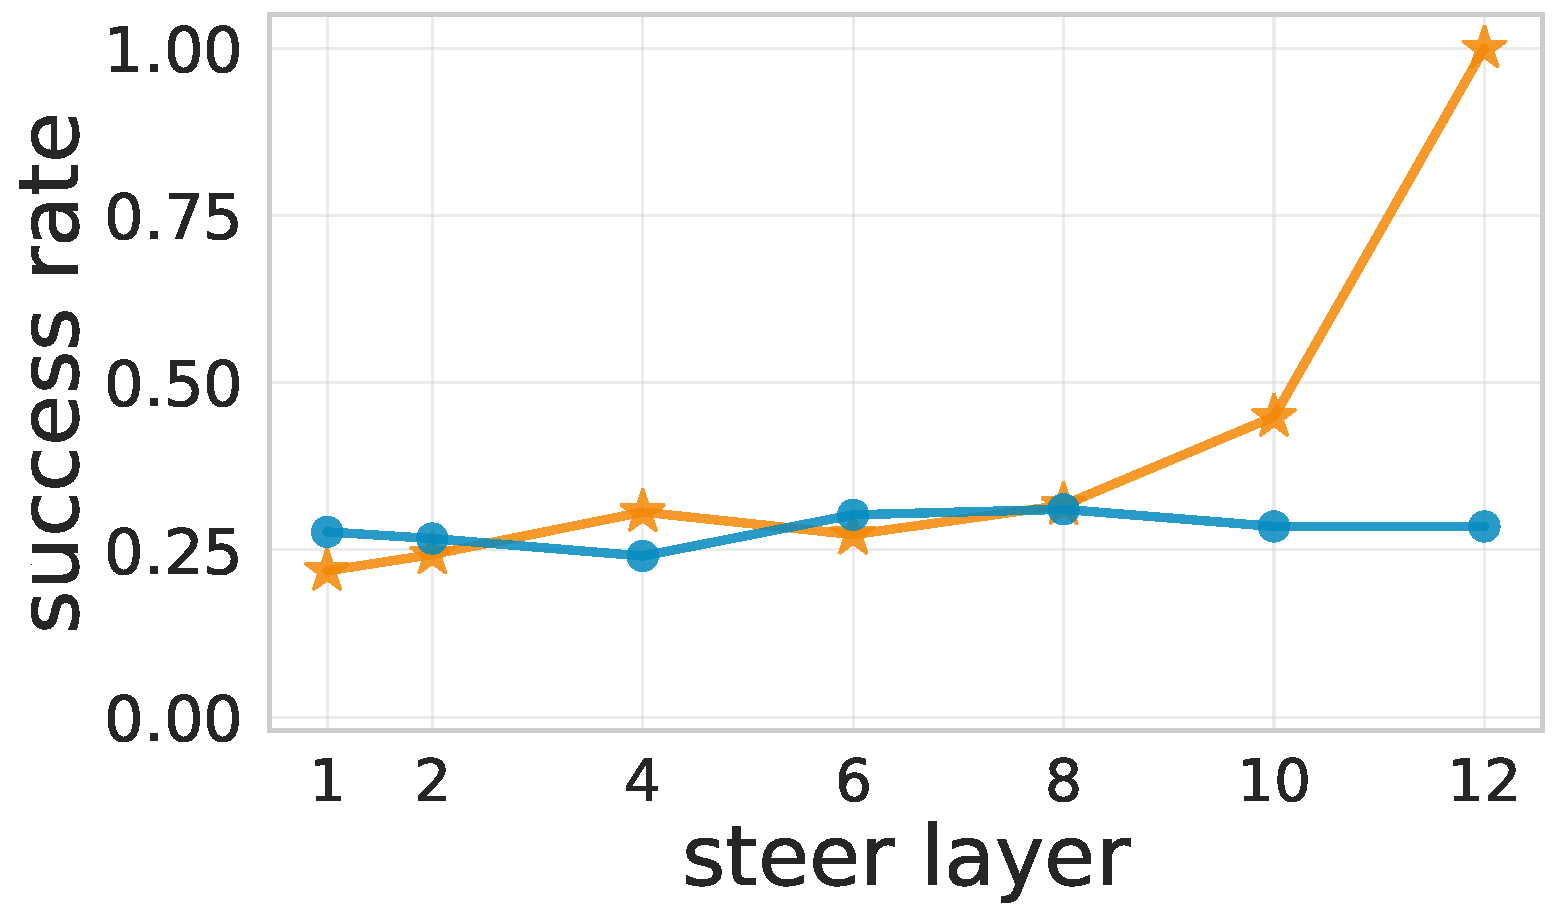
\includegraphics[width=\linewidth]{results_steer_layers/by_layer_atom_type.pdf}
    \subcaption{atom type}
    \label{fig:steer-all-atom-type}
\end{subfigure}\hfill
\begin{subfigure}[t]{0.48\linewidth}
    \centering
    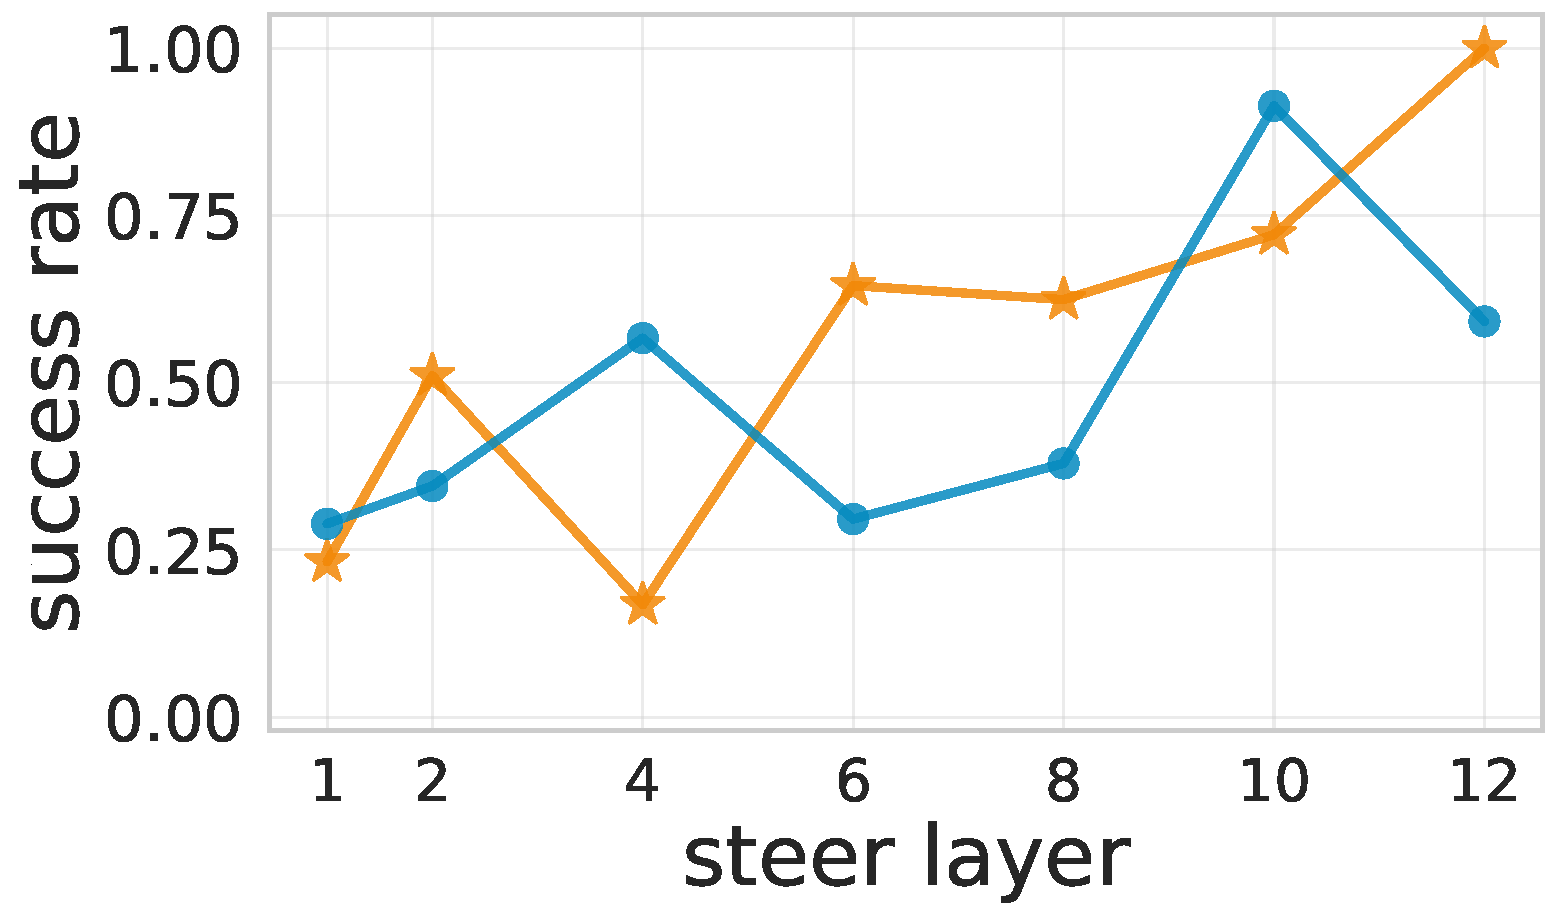
\includegraphics[width=\linewidth]{results_steer_layers/by_layer_hybridization.pdf}
    \subcaption{hybridization}
    \label{fig:steer-all-hybridization}
\end{subfigure}

\vspace{0.6em}

\begin{subfigure}[t]{0.48\linewidth}
    \centering
    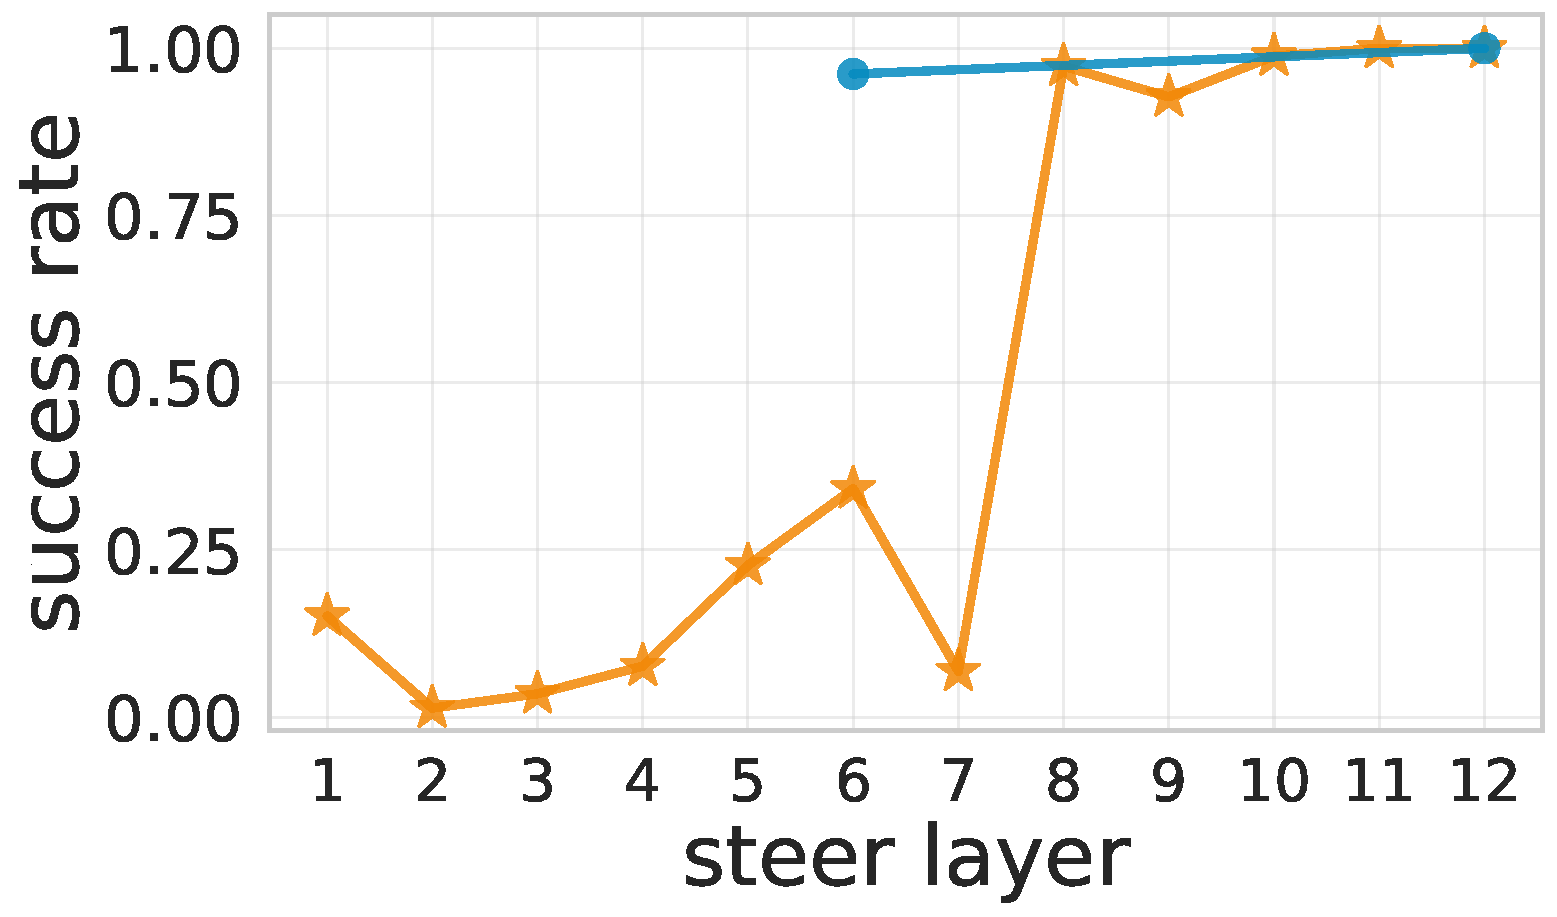
\includegraphics[width=\linewidth]{results_steer_layers/by_layer_formal_charge.pdf}
    \subcaption{formal charge}
    \label{fig:steer-all-formal-charge}
\end{subfigure}\hfill
\begin{subfigure}[t]{0.48\linewidth}
    \centering
    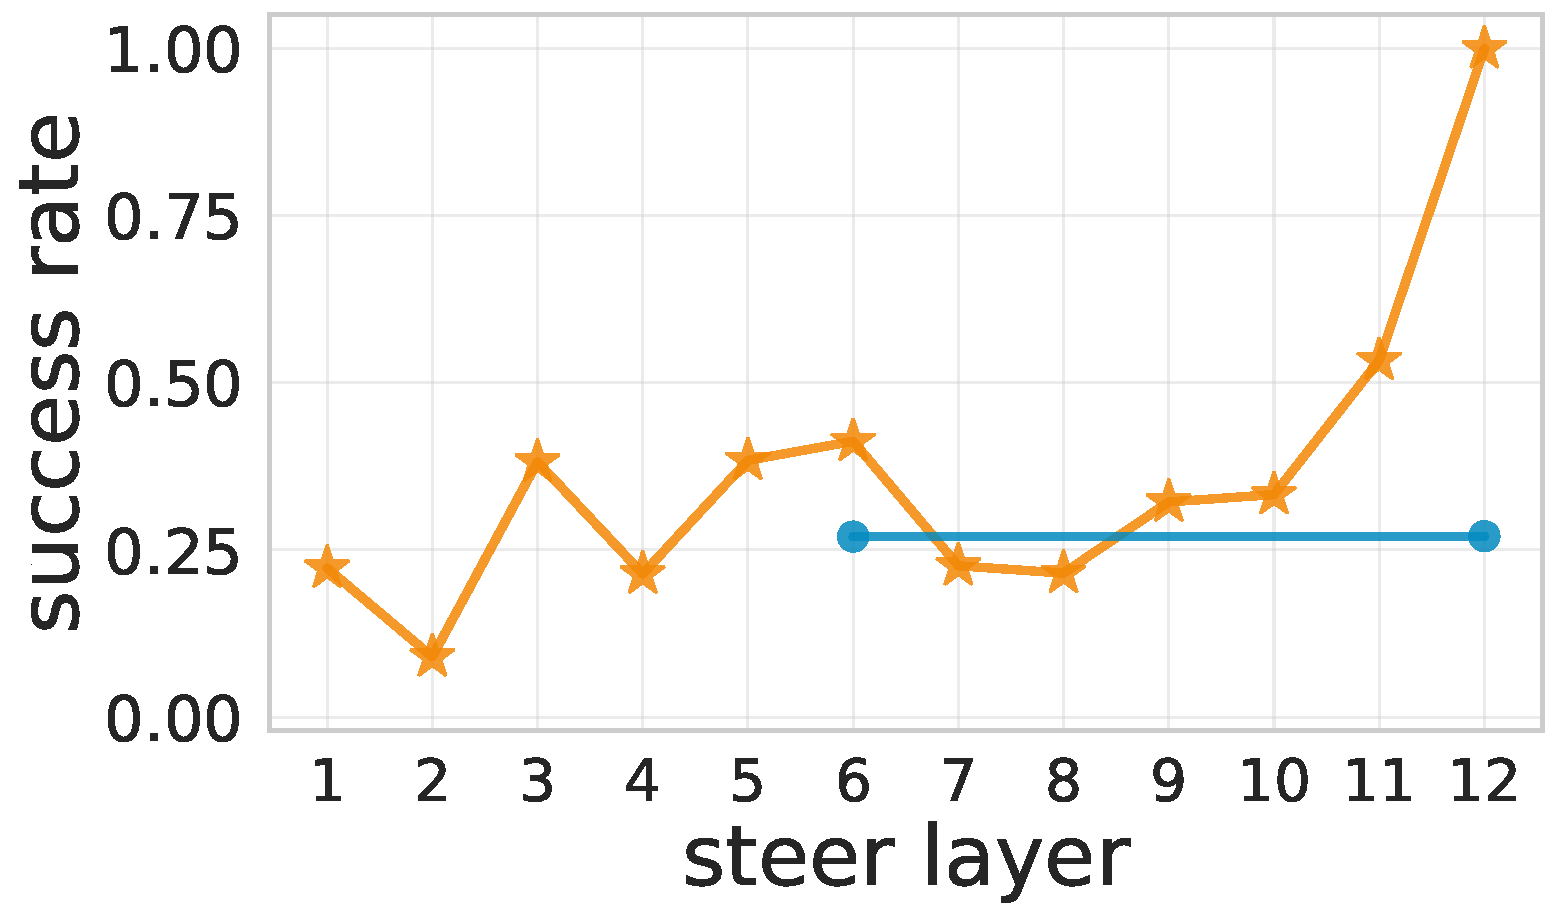
\includegraphics[width=\linewidth]{results_steer_layers/by_layer_total_valence.pdf}
    \subcaption{total valence}
    \label{fig:steer-all-total-valence}
\end{subfigure}

\vspace{0.4em}

\centerline{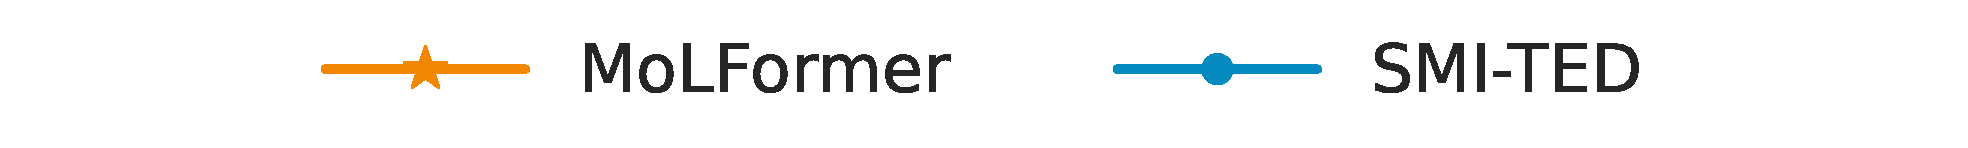
\includegraphics[width=0.5\linewidth]{results_steer_layers/by_layer_legend.pdf}}

\caption{Intervention success rate as a function of the steer layer for the four properties not shown in the main text. Formal charge (\ref{fig:steer-all-formal-charge}) follows the same pretraining-difference shape seen in the main text: \smi saturates at high success by mid-layers, \molm climbs gradually until the top of the encoder. Atom type (\ref{fig:steer-all-atom-type}), hybridization (\ref{fig:steer-all-hybridization}), and total valence (\ref{fig:steer-all-total-valence}) are multi-class targets and the cycle-target success rate is partly governed by the probe-prototype layout; we therefore additionally inspect the moved-off-source rate (Appendix~\ref{app:steering}) to disentangle ``the intervention had effect'' from ``the intervention hit the cycle target''.}
\label{fig:steer-layer-all}
\end{figure}
